\section{Plate Vibration and Radiated Sound Power}

A thin, flat plate that is simply supported along its edges vibrates in a set of characteristic shapes, called mode shapes, each with its own natural frequency \parencite{leissa1969plate,timoshenko1959plate}. The plate used throughout this thesis is rectangular, with length $L_x = 1.4\,\si{\meter}$, width $L_y = 0.5\,\si{\meter}$ and thickness $h = 0.005\,\si{\meter}$, made of an aluminium-like material with Young's modulus $E = 71\,\si{\giga\pascal}$ (with a small structural loss factor), density $\rho = 2800\,\si{\kilo\gram\per\cubic\meter}$ and Poisson's ratio $\nu = 0.3$. Its bending behaviour is governed by the Kirchhoff--Love thin-plate equation, with point forces added at the excitation point and at every resonator attachment:
\begin{equation}
D \nabla^4 w + \rho h \ddot w = f_d(t)\,\delta(x-x_d)\delta(y-y_d) - \sum_{i=1}^{R} \delta(x-x_i)\delta(y-y_i)\big[k_i(w-u_i) + c_i(\dot w - \dot u_i)\big],
\end{equation}
where $w(x,y,t)$ is the plate's transverse displacement, $D = Eh^3/(12(1-\nu^2))$ is the plate's bending stiffness, $f_d(t)$ is a point force at $(x_d,y_d)$, and the sum adds the coupling force of every one of the $R$ resonators attached at $(x_i,y_i)$. Each resonator is itself a mass $m_i$ on a spring $k_i$ and a damper $c_i$, driven by the plate's motion at its own attachment point:
\begin{equation}
m_i \ddot u_i + c_i(\dot u_i - \dot w_i) + k_i(u_i - w_i) = 0, \qquad w_i = w(x_i, y_i, t), \qquad i = 1, \dots, R,
\end{equation}
with $u_i$ the resonator's own displacement.

For a simply supported rectangular plate, the displacement is written as a weighted sum of mode shapes,
\begin{equation}
w(x,y,t) = \sum_{m,n} q_{mn}(t)\,\phi_{mn}(x,y), \qquad \phi_{mn}(x,y) = \frac{2}{\sqrt{\rho h L_x L_y}}\sin\!\Big(\frac{m\pi x}{L_x}\Big)\sin\!\Big(\frac{n\pi y}{L_y}\Big),
\end{equation}
with natural frequencies $\omega_{mn} = \sqrt{D/(\rho h)}\big[(m\pi/L_x)^2 + (n\pi/L_y)^2\big]$. This is called modal superposition, or the normal mode approach \parencite{gavric1993sti}, and it is the basis of the physics solver used throughout this thesis: instead of solving for the plate's motion at every point directly, the solver finds the modal weight $q_{mn}(t)$ of each kept mode and then combines the mode shapes to get the motion anywhere on the plate. Only a finite number of modes, $N$, can be kept; this thesis uses as many as the forward and invertible models need to represent the frequency range of interest, which is stated together with every dataset in Chapter~\ref{ch:concept}. Combining the plate and the $R$ resonators into one coupled system and solving in the frequency domain gives
\begin{equation}
\big(\mathbf K + j\omega\,\mathbf C - \omega^2 \mathbf M\big)\, \hat{\mathbf w}(\omega) = \hat{\mathbf f},
\end{equation}
a system of $N+R$ equations that is solved at every excitation frequency $\omega = 2\pi f$ of interest.

Once the plate's vibration is known, the sound power it radiates into the surrounding air can be estimated directly from the plate's surface velocity $\mathbf v = j\omega\mathbf w$, without solving a separate acoustic problem for the air itself:
\begin{equation}
P(f) = \frac{1}{2}\rho_f c_f \int_A |\mathbf v(f)|^2 \, \mathrm dA, \qquad \mathrm{ERP}(f) = 10 \log_{10}\frac{P(f)}{P_\text{ref}}, \qquad P_\text{ref} = 10^{-12}\,\si{\watt},
\end{equation}
with $\rho_f = 1.21\,\si{\kilo\gram\per\cubic\meter}$ the density of air and $c_f = 343\,\si{\meter\per\second}$ the speed of sound. This estimate, the equivalent radiated power (ERP) \parencite{luegmair2015advanced}, is a good approximation of the true radiated power for a plate that is small compared to the acoustic wavelength, which holds for the frequency range used in this thesis. The ERP is reported in decibels and is the single quantity this thesis trains its models to predict and, eventually, to control.

Several resonators placed at different points couple to different mode shapes by different amounts, depending on their position, so where a resonator sits matters as much as what it is tuned to.

\section{Neural Operators}

A standard neural network learns a mapping between two fixed-size vectors. A neural operator \parencite{kovachki2023neural} instead learns a mapping between two functions, for example between a resonator design and the sound power spectrum it produces at every frequency in a range. Because the mapping is learned from many examples rather than derived from physical equations, a trained neural operator can evaluate a new design in a fraction of a second, instead of the time a full physics solve takes. This speed is what makes it practical to search over many designs, which is needed for generative design. The forward architectures compared in Chapter~\ref{ch:concept} are different ways of building such a mapping.

\section{Invertibility and Generative Design}

A regular neural operator only works in one direction: from a design to a spectrum. Generative design needs the other direction too: from a target spectrum to a design that would produce it. One way to get both directions from a single trained model is to build the network out of blocks that are mathematically invertible, so that running the network backward through the same blocks recovers the input from the output. This thesis uses two such building blocks: a coupling block \parencite{dinh2017realnvp}, which splits its input in two halves and transforms one half using the other, and can be undone step by step; and an invertible DeepONet \parencite{kaltenbach2023invertible}, which makes the operator's branch network itself one of these invertible blocks.

Because the mapping from a spectrum to a design is rarely unique, several genuinely different designs can produce a very similar spectrum. Figure~\ref{fig:non-unique} shows a real example found in the three-resonator dataset used in this thesis: two configurations with completely different resonator masses, positions and tuning frequencies, whose solver-computed ERP spectra agree to 0.4\,dB RMSE across the whole frequency range, and differ by at most 3.0\,dB, in a narrow notch near 37\,Hz that one resonator of the first configuration produces. The pair was found by searching the dataset for configurations with nearly identical spectra and keeping the pair whose designs differ most. An inverse model has no way to tell these two designs apart from the spectrum alone. For this reason, the invertible models in this thesis also include a variational step that turns a single proposed design into a small family of plausible designs, instead of just one guess.

\begin{figure}[h]
\centering
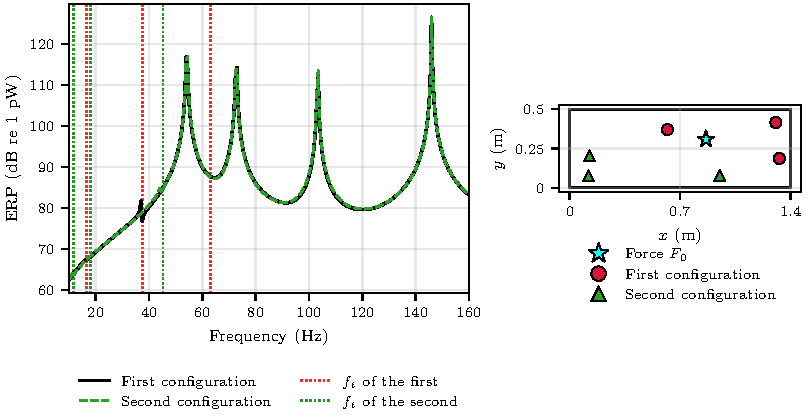
\includegraphics[max width=\textwidth]{Bilder/same_erp_different_resonators.pdf}
\caption[Two different designs with nearly the same ERP spectrum]{Two genuinely different three-resonator designs (different masses, positions and tuning frequencies) whose solver-computed ERP spectra are nearly identical (RMSE 0.39\,dB). Left: the two spectra overlaid, with the tuning frequencies of the resonators as dotted lines. Right: both resonator layouts on the plate, numbered by increasing tuning frequency.}
\label{fig:non-unique}
\end{figure}

\section{Uncertainty Quantification over Manufacturing Tolerances}

A design that looks good on paper is never built exactly as specified: a resonator's mass, position or tuning will always be off by a small amount once it is actually manufactured. Monte Carlo uncertainty quantification \parencite{metropolis1949monte} checks how much this matters. A chosen design is perturbed many times by small random amounts that match realistic manufacturing tolerances, for example a mass that is accurate to within two percent, and each perturbed version is evaluated with the fast forward surrogate. Collecting the resulting spectra gives a spread, instead of a single curve, which shows how sensitive a proposed design's acoustic behaviour is to the small errors that manufacturing will inevitably introduce. This only works with a fast surrogate model, since it needs many evaluations of the same design region, far more than the physics solver could provide in reasonable time.
